\documentclass[11pt]{article}

\usepackage[margin=1in]{geometry}
\usepackage[T1]{fontenc}
\usepackage{lmodern}
\usepackage{microtype}
\usepackage{amsmath,amssymb,amsthm}
\usepackage{booktabs}
\usepackage{graphicx}
\usepackage{subcaption}
\usepackage{xcolor}
\usepackage{pgfplots}
\usepackage{pgfplotstable}
\usepackage[numbers,sort&compress]{natbib}
\usepackage[hidelinks]{hyperref}

\pgfplotsset{compat=1.18}
\usetikzlibrary{patterns}

\newtheorem{proposition}{Proposition}

\newcommand{\hM}{h_{\mathrm{M}}}
\newcommand{\hE}{h_{\mathrm{E}}}
\newcommand{\hA}{h_{\mathrm{A}}}
\newcommand{\hMA}{h_{\mathrm{M+A}}}
\newcommand{\hAbs}{h_{|\Delta|}}

\title{\Huge\bfseries How Much Does a Heuristic Buy?\\[6pt]
\Large\bfseries A* versus Branch and Bound for Least-Effort Walking Routes on Terrain Maps}

\author{Abdulla Alfalasi\\
\small COM1005 coursework, University of Sheffield (May 2021)\\
\small \url{https://github.com/aalbudoor/astar-vs-branch-and-bound}}

\date{}

\begin{document}
\maketitle

\begin{abstract}
A rambler crosses a height map one cell at a time. Level or downhill steps cost 1, and climbing costs 1 plus the height gained. We compare branch and bound (uniform-cost search) with A* under five heuristics on the 16$\times$16 course map and three seeded 64$\times$64 synthetic terrains, using 500 random start/goal pairs in total. Four heuristics never overestimate the remaining cost: straight-line distance, Manhattan distance, remaining ascent, and Manhattan distance plus remaining ascent. The fifth, absolute height difference, can overestimate it. All four admissible heuristics returned an optimal route in every run. The combined heuristic did best everywhere. It expanded 25\% of the nodes branch and bound expanded on smooth terrain, but 72\% on rugged terrain, and a simple informedness measure, $h(\text{start})/C^*$, tracks this gap. The absolute-height heuristic returned a suboptimal route in 22--56\% of pairs. On the two noisier 64$\times$64 maps it also expanded more nodes than branch and bound, because it repeatedly reopened closed nodes.
\end{abstract}

\section{Introduction}
Path planning over terrain is a standard testbed for informed search. The textbook claim is that A* with an admissible heuristic finds the same optimal path as an uninformed method such as branch and bound or Dijkstra's algorithm \citep{dijkstra1959note,lawler1966branch}, while expanding fewer nodes \citep{hart1968formal,dechter1985generalized}. How many fewer depends on how much of the true cost the heuristic captures, and that in turn depends on the terrain.

This report asks three questions:
\begin{enumerate}
  \item How many node expansions does each heuristic save relative to branch and bound, and how does this change with the terrain?
  \item Does combining distance and ascent information help, and can the gain be predicted from the heuristic alone?
  \item What does an inadmissible heuristic cost in route quality and in search effort?
\end{enumerate}

\section{Problem}
A terrain map is a grid of heights $H(r,c) \in \{0,\dots,255\}$. A state is a cell $(r,c)$, and the rambler can move to any of its four neighbours. The cost of stepping from cell $u$ to a neighbouring cell $v$ is
\begin{equation}
  c(u,v) =
  \begin{cases}
    1 & \text{if } H(v) \le H(u),\\
    1 + H(v) - H(u) & \text{if } H(v) > H(u),
  \end{cases}
  \label{eq:cost}
\end{equation}
so descending is as cheap as walking on the flat and every metre climbed is paid for. The task is to find a path of least total cost $C^*$ from a start cell to a goal cell.

\section{Methods}

\subsection{Search algorithms}
Both algorithms keep an \emph{open} list of generated nodes and a \emph{closed} list of expanded nodes. A node records its state, its cost so far $g$, and its parent. When a successor reaches a state already on open or closed by a cheaper route, that node is updated and, if it was closed, moved back to open. Search stops when a goal node is \emph{selected} for expansion, not when it is generated, which is what makes the returned path optimal.

\paragraph{Branch and bound} always selects the open node with the lowest $g$. With the duplicate check above it is uniform-cost search, the node-selection form of Dijkstra's algorithm \citep{dijkstra1959note,russell2020aima}.

\paragraph{A*} selects the open node with the lowest $f = g + h$, where $h$ estimates the remaining cost to the goal \citep{hart1968formal}. With $h \equiv 0$ it reduces to branch and bound. We checked this in the code: on every instance tested, A* with $h \equiv 0$ reproduced branch and bound's path cost and node count exactly.

\subsection{Heuristics}
Let $(r,c)$ be the current cell and $(r_g,c_g)$ the goal. Table~\ref{tab:heuristics} lists the five heuristics compared.

\begin{table}[t]
\centering
\caption{Heuristics compared. ``Admissible'' means the heuristic never exceeds the true remaining cost.}
\label{tab:heuristics}
\begin{tabular}{llc}
\toprule
Name & Definition & Admissible \\
\midrule
Euclidean $\hE$ & $\lfloor \sqrt{(r-r_g)^2 + (c-c_g)^2} \rfloor$ & yes \\
Manhattan $\hM$ & $|r-r_g| + |c-c_g|$ & yes \\
Ascent $\hA$ & $\max\bigl(0,\; H(r_g,c_g) - H(r,c)\bigr)$ & yes \\
Manhattan+Ascent $\hMA$ & $\hM + \hA$ & yes \\
Absolute height $\hAbs$ & $|H(r_g,c_g) - H(r,c)|$ & no \\
\bottomrule
\end{tabular}
\end{table}

\begin{proposition}
$\hMA$ is admissible and consistent, and it dominates $\hM$, $\hE$ and $\hA$.
\end{proposition}
\begin{proof}
Write each step cost in~\eqref{eq:cost} as $1 + \max(0, \Delta)$, where $\Delta$ is the height change of the step. Any path from $u$ to the goal has at least $\hM(u)$ steps. Its positive height changes sum to at least the net rise $H(\text{goal}) - H(u)$, and to at least 0. The path therefore costs at least $\hM(u) + \hA(u) = \hMA(u)$, which proves admissibility. For consistency, take one step from $u$ to $v$. Then $\hM(u) \le 1 + \hM(v)$. The inequality $\max(0, a+b) \le \max(0,a) + \max(0,b)$ gives $\hA(u) \le \max(0, H(v)-H(u)) + \hA(v)$. Adding the two gives $\hMA(u) \le c(u,v) + \hMA(v)$. Dominance holds because $\hA \ge 0$, $\hM \ge 0$ and $\hE \le \hM$.
\end{proof}

$\hAbs$ looks like a natural ``height difference'' heuristic, but it also charges for descents, which are cheap: a single downhill step of 100 costs 1, yet $\hAbs$ estimates it at 100. By standard results, a consistent heuristic that dominates another expands no more nodes, ignoring ties \citep{pearl1984heuristics,dechter1985generalized}. We therefore expect $\hMA$ to expand the fewest nodes of the admissible heuristics. No such guarantee applies to $\hAbs$.

\section{Experimental Setup}

\paragraph{Maps.}
We use the 16$\times$16 map \texttt{tmc.pgm} supplied with the coursework, and three 64$\times$64 maps generated as sums of Gaussian hills with per-cell Gaussian noise, rescaled to 0--255 (Table~\ref{tab:maps}). The three maps range from a few broad hills to many narrow, noisy ones.

\begin{table}[t]
\centering
\caption{Terrain maps. Synthetic maps are regenerated from the listed seed by \texttt{TerrainGenerator}.}
\label{tab:maps}
\begin{tabular}{lccccc}
\toprule
Map & Size & Hills & Hill width $\sigma$ & Noise s.d. & Pairs \\
\midrule
\texttt{tmc16} (course map) & 16$\times$16 & --- & --- & --- & 200 \\
\texttt{smooth64} & 64$\times$64 & 8 & 8--16 & 0 & 100 \\
\texttt{rolling64} & 64$\times$64 & 30 & 3--8 & 4 & 100 \\
\texttt{rugged64} & 64$\times$64 & 120 & 1.5--4 & 12 & 100 \\
\bottomrule
\end{tabular}
\end{table}

\paragraph{Instances.}
For each map we sampled start/goal pairs uniformly at random with a fixed seed. We kept only pairs at least half the map width apart in Manhattan distance, which excludes trivial instances. Every method ran on the same pairs.

\paragraph{Metrics.}
\emph{Nodes expanded} counts every selection from open, including re-expansions of reopened nodes. We report it relative to branch and bound on the same pair and average the ratio over pairs. \emph{Optimality} compares each path's cost with branch and bound's, which is optimal. \emph{Informedness} is $h(\text{start})/C^*$, the fraction of the true cost the heuristic sees before the search begins. We also give the coursework's \emph{efficiency} measure, path length divided by nodes expanded. Wall-clock time is recorded, but open and closed are linear-scan lists, so time mostly tracks node count.

\paragraph{Implementation.}
The search engine (\texttt{Search}, \texttt{SearchNode}, \texttt{SearchState}, \texttt{TerrainMap}) is the COM1005 base code by Phil Green and Heidi Christensen. The Ramblers state, the heuristics, the terrain generator and the experiment harness are ours. The code is Java 8 compatible, and \texttt{run\_experiments.sh} regenerates every number and figure in this report. Apart from timing, the results are deterministic.

\section{Results}

\subsection{Search effort and optimality}
Table~\ref{tab:main} and Figure~\ref{fig:ratio} summarize the 500 pairs. All four admissible heuristics returned an optimal route on every pair of every map, as the theory predicts. Their savings differ widely.

\begin{table}[t]
\centering
\caption{Mean nodes expanded relative to branch and bound (lower is better), percentage of pairs solved optimally, and mean and maximum cost excess over the optimum. Branch and bound's own mean expansions are 148, 2360, 2622 and 2797 for the four maps.}
\label{tab:main}
\small
\begin{tabular}{l cc cc cc cc}
\toprule
& \multicolumn{2}{c}{\texttt{tmc16}} & \multicolumn{2}{c}{\texttt{smooth64}} & \multicolumn{2}{c}{\texttt{rolling64}} & \multicolumn{2}{c}{\texttt{rugged64}} \\
\cmidrule(lr){2-3}\cmidrule(lr){4-5}\cmidrule(lr){6-7}\cmidrule(lr){8-9}
Method & ratio & opt.\,\% & ratio & opt.\,\% & ratio & opt.\,\% & ratio & opt.\,\% \\
\midrule
Branch and bound & 1.00 & 100 & 1.00 & 100 & 1.00 & 100 & 1.00 & 100 \\
A* Euclidean     & 0.83 & 100 & 0.57 & 100 & 0.74 & 100 & 0.85 & 100 \\
A* Manhattan     & 0.79 & 100 & 0.45 & 100 & 0.66 & 100 & 0.81 & 100 \\
A* Ascent        & 0.79 & 100 & 0.82 & 100 & 0.81 & 100 & 0.91 & 100 \\
A* Manhattan+Ascent & \textbf{0.56} & 100 & \textbf{0.25} & 100 & \textbf{0.48} & 100 & \textbf{0.72} & 100 \\
A* Abs.\ height  & 0.76 & 71 & 0.71 & 78 & 1.11 & 44 & 1.10 & 63 \\
\midrule
\multicolumn{9}{l}{Cost excess of A* Abs.\ height over optimum: mean / max (\%)} \\
& \multicolumn{2}{c}{16.9 / 455} & \multicolumn{2}{c}{2.7 / 51} & \multicolumn{2}{c}{7.5 / 126} & \multicolumn{2}{c}{1.9 / 22} \\
\bottomrule
\end{tabular}
\end{table}

\begin{figure}[t]
\centering
\begin{tikzpicture}
\begin{axis}[
  width=\linewidth, height=6.2cm,
  ybar, bar width=5.5pt, area legend,
  ymin=0, ymax=1.25,
  ylabel={Nodes expanded / branch and bound},
  symbolic x coords={tmc16,smooth64,rolling64,rugged64},
  xtick=data,
  x tick label style={font=\ttfamily\small},
  enlarge x limits=0.15,
  legend style={font=\footnotesize, at={(0.5,1.03)}, anchor=south, legend columns=3, draw=none},
  ymajorgrids, grid style={gray!25},
  extra y ticks={1}, extra y tick style={grid=major, grid style={black, dashed}},
]
\addplot[fill=gray!55, draw=gray!80] table[x=map, y=euclidean, col sep=comma] {../results/expanded_ratio_wide.csv};
\addplot[fill=blue!45, draw=blue!70] table[x=map, y=manhattan, col sep=comma] {../results/expanded_ratio_wide.csv};
\addplot[fill=teal!45, draw=teal!70] table[x=map, y=ascent, col sep=comma] {../results/expanded_ratio_wide.csv};
\addplot[fill=orange!75, draw=orange!90!black] table[x=map, y=manhattan_ascent, col sep=comma] {../results/expanded_ratio_wide.csv};
\addplot[fill=red!55, draw=red!80!black, postaction={pattern=north east lines}] table[x=map, y=abs_height, col sep=comma] {../results/expanded_ratio_wide.csv};
\legend{Euclidean, Manhattan, Ascent, Manhattan+Ascent, Abs.\ height (inadmissible)}
\end{axis}
\end{tikzpicture}
\caption{Mean nodes expanded by A* relative to branch and bound (dashed line). Manhattan+Ascent expands the fewest nodes on every map. The inadmissible absolute-height heuristic does worse than branch and bound on the two noisier 64$\times$64 maps.}
\label{fig:ratio}
\end{figure}

Manhattan+Ascent was the best heuristic on every map. On \texttt{smooth64} it expanded a quarter of the nodes branch and bound expanded, and its mean search time fell from 22.4\,ms to 2.0\,ms in our run (timings vary from run to run; node counts do not). Distance alone mattered more than ascent alone on the synthetic maps. On the small course map the two did equally well (0.79), and adding them together gave far more than either alone. The ordering $\hMA < \hM < \hE$ in nodes expanded matches the dominance ordering of the three heuristics.

\subsection{Why the savings shrink on rugged terrain}
The gain from every heuristic fell as the terrain became rougher: Manhattan+Ascent went from 0.25 on \texttt{smooth64} to 0.72 on \texttt{rugged64}. Table~\ref{tab:informedness} shows why. On smooth terrain the optimal route is close to a straight walk plus the unavoidable climb, so $\hMA$ sees 79\% of the true cost from the start. On rugged terrain the optimal route pays for many small climbs and detours that no local estimate can see, and $\hMA$ sees only 27\%. Across the three synthetic maps, which share a size, lower informedness goes with a higher expansion ratio for every admissible heuristic except Ascent, whose informedness is low everywhere. Unlike the expansion ratio, informedness can be measured from a sample of solved instances without comparing search runs.

\begin{table}[t]
\centering
\caption{Mean informedness $h(\text{start})/C^*$ of each heuristic. Values above 1 mean the heuristic overestimates.}
\label{tab:informedness}
\begin{tabular}{lcccc}
\toprule
Heuristic & \texttt{tmc16} & \texttt{smooth64} & \texttt{rolling64} & \texttt{rugged64} \\
\midrule
Euclidean & 0.20 & 0.49 & 0.27 & 0.15 \\
Manhattan & 0.27 & 0.64 & 0.35 & 0.20 \\
Ascent & 0.24 & 0.15 & 0.13 & 0.07 \\
Manhattan+Ascent & 0.51 & 0.79 & 0.48 & 0.27 \\
Abs.\ height & 1.72 & 0.63 & 0.44 & 0.16 \\
\bottomrule
\end{tabular}
\end{table}

\subsection{The cost of an inadmissible heuristic}
The absolute-height heuristic returned a suboptimal route on 22--56\% of pairs. The worst route on the course map cost 61 against an optimum of 11, 5.5 times as much. It was also not reliably faster. On \texttt{rolling64} and \texttt{rugged64} it expanded about 10\% \emph{more} nodes than branch and bound, and on one \texttt{rolling64} pair it expanded 20{,}047 nodes on a 4{,}096-cell map. An inconsistent heuristic can close a node by an expensive route and then find a cheaper one. The node is then reopened and expanded again, and those re-expansions add up. On the course map it has a mean informedness of 1.72, so it usually overestimates, and its apparent savings there come largely from that overestimation. It prunes aggressively by ignoring routes that are actually cheap.

\subsection{Example}
Figure~\ref{fig:example} shows one pair on \texttt{smooth64}. All four methods returned routes of cost 95. Branch and bound expanded 3322 nodes, most of the map. Manhattan expanded 1221 and Manhattan+Ascent 1148, both confined to a corridor around the route. The absolute-height heuristic still found the optimum here but expanded 4662 nodes, more than the map contains, because of re-expansions.

\begin{figure}[t]
\centering
\begin{subfigure}{0.24\linewidth}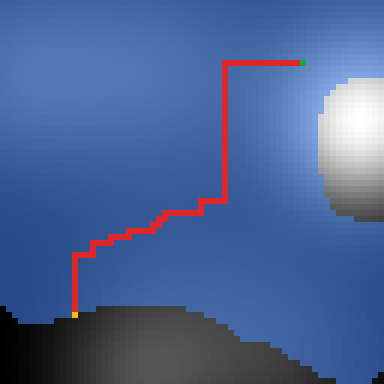
\includegraphics[width=\linewidth]{../results/figures/example_BranchAndBound.png}\caption{Branch and bound\\3322 expanded}\end{subfigure}\hfill
\begin{subfigure}{0.24\linewidth}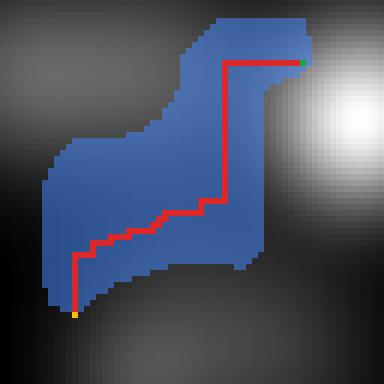
\includegraphics[width=\linewidth]{../results/figures/example_AStar-Manhattan.png}\caption{A* Manhattan\\1221 expanded}\end{subfigure}\hfill
\begin{subfigure}{0.24\linewidth}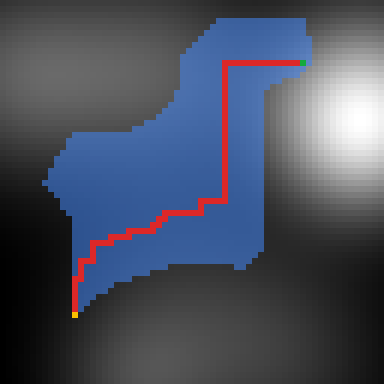
\includegraphics[width=\linewidth]{../results/figures/example_AStar-Manhattan+Ascent.png}\caption{A* Manh.+Ascent\\1148 expanded}\end{subfigure}\hfill
\begin{subfigure}{0.24\linewidth}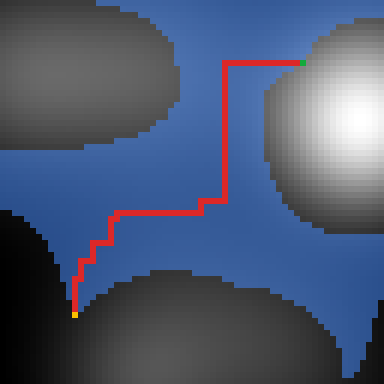
\includegraphics[width=\linewidth]{../results/figures/example_AStar-AbsHeight.png}\caption{A* Abs.\ height\\4662 expanded}\end{subfigure}
\caption{Start (green, top right) to goal (yellow, bottom left) on \texttt{smooth64}; lighter cells are higher. Blue cells were expanded and the red line is the route found. All four routes cost 95.}
\label{fig:example}
\end{figure}

\section{Discussion and Limitations}
The practical lesson is to build the heuristic from the cost function. Each step in this problem pays for distance and for climbing, and the heuristic that bounds both terms beat the two that bound only one. Informedness is a cheap diagnostic: it can be computed from a sample of solved instances before choosing a heuristic, and on the synthetic maps it tracked the terrain effect.

The study has several limitations. The synthetic maps come from one generator with one seed per roughness level, so the terrain effect is shown on three maps, not a distribution of them. Movement is 4-connected, and diagonal moves would change both the costs and which heuristics are admissible. Open and closed are linear lists, as in the base code, so timings would shrink with a priority queue and a hash set. The node-count comparisons would not change. Ties in $f$ are broken by list order, which can shift node counts slightly between heuristics with equal $f$ values.

\section{Conclusion}
On least-effort terrain routing, A* with any admissible heuristic returned the same optimal routes as branch and bound, and it expanded between 25\% and 91\% as many nodes, depending on the heuristic and the terrain. A heuristic that combines Manhattan distance with remaining ascent is admissible and consistent, and it was the best choice on every map. Its advantage shrinks on rugged terrain, as its informedness predicts. The absolute-height heuristic is not admissible. It returned suboptimal routes on up to 56\% of pairs, and on the two noisier 64$\times$64 maps it searched more than branch and bound did.

\section*{Acknowledgements}
The search framework and terrain map reader are the COM1005 base code written by Phil Green (2013) and Heidi Christensen (2021) at the University of Sheffield.

\bibliographystyle{plainnat}
\bibliography{references}

\end{document}
